\documentclass[alpha-refs]{wiley-article}

% --- Journal Provided

\usepackage{url}
\usepackage{lineno}
\usepackage{soul}

\usepackage{graphicx}
\usepackage[space]{grffile}
\usepackage{latexsym}
\usepackage{textcomp}
\usepackage{longtable}
\usepackage{tabulary}
\usepackage{booktabs,array,multirow}
\usepackage{amsfonts,amsmath,amssymb}
\usepackage{natbib}
\usepackage{etoolbox}
\makeatletter
% This gives an error ...
%\patchcmd\@combinedblfloats{\box\@outputbox}{\unvbox\@outputbox}{}{%
%  \errmessage{\noexpand\@combinedblfloats could not be patched}%
%}%
\makeatother
% You can conditionalize code for latexml or normal latex using this.
\newif\iflatexml\latexmlfalse
\providecommand{\tightlist}{\setlength{\itemsep}{0pt}\setlength{\parskip}{0pt}}%

\AtBeginDocument{\DeclareGraphicsExtensions{.pdf,.PDF,.eps,.EPS,.png,.PNG,.tif,.TIF,.jpg,.JPG,.jpeg,.JPEG}}

\usepackage[utf8]{inputenc}
\usepackage[english]{babel}

% --- Custom additions
\usepackage{mathtools} % for \coloneqq
\usepackage{color}
\usepackage{bm}
\usepackage{adjustbox}
\usepackage[percent]{overpic}


% Definitions
\usepackage{ide}

\usepackage{hyperref}
\hypersetup{colorlinks=false,pdfborder={0 0 0}}
\usepackage[capitalise,noabbrev]{cleveref}

\newcommand{\red}[1]{\textcolor{red}{#1}}
\newcommand{\blue}[1]{\textcolor{blue}{#1}}

% Define some citation abbreviations
\defcitealias{RSSB:RSSB777}{L11}

% From qjrms
\renewcommand{\sfdefault}{ptm}
\renewcommand{\familydefault}{\sfdefault}
\papertype{Original Article}

% --- Header
\title{A Practical Formulation for an Anisotropic and Nonstationary Mat\'ern Class
    Correlation Operator
}
\author[1,2,3]{Timothy A. Smith}

\affil[1]{Cooperative Institute for Research in Environmental Sciences
    (CIRES) at the University of Colorado Boulder, Boulder, CO, USA
}
\affil[2]{Physical Sciences Laboratory (PSL), National Oceanic and
    Atmospheric Administration (NOAA), Boulder, CO, USA
}
\affil[3]{Oden Institute for Computational Engineering and Sciences,
    The University of Texas at Austin, Austin, TX, USA
}

\corraddress{Timothy A. Smith, David Skaggs Research Center, Boulder, CO, 80305,
    USA
}
\corremail{tim.smith@noaa.gov}

\fundinginfo{This work was funded in part by
    NASA NNH19ZDA001N-SLCST
    and a JPL/Caltech Subcontract (ECCO Consortium)
}

\runningauthor{Timothy A. Smith}

\begin{document}

\maketitle
\begin{abstract}
    A key component of data assimilation methods is the specification of
    univariate spatial correlations, which appear in the background-error
    covariance.
    For realistic problems in meteorology and oceanography,
    correlation length scales are nonstationary (variable in space) and
    anisotropic (variable in each direction).
    Variational approaches typically use an operator to enforce correlation
    length scales, and thus the operator must be designed to capture
    desired levels of nonstationarity and anisotropy.
    For systems with complex boundaries, such as the ocean, it is natural
    to use a filtering approach based on the application of an elliptic,
    Laplacian-like operator.
    Here we show how an elliptic operator can be formulated to capture a general
    Mat\'ern-type correlation structure.
    We show how nonstationarity and anisotropy can be encoded into the operator
    via a simple change of variables based on user-defined
    normalization length scales.
    The change of variables defines a mapping between the computational domain
    and a space where the analytical Mat\'ern correlation function
    applies.
    In addition to the mapping, two other hyperparameters \textit{separately}
    control the correlation length scale (i.e.\ range) and shape.
    As a practical use-case, we apply the operator to a global ocean model.
    We show that when the normalizing length scales correspond to the local grid
    scale, the range parameter has an intuitive
    interpretation as the number of neighboring grid cells at which correlation drops to 0.14.
    Finally, the correlation model is shown to be computationally efficient in
    two regards.
    First, the necessary linear solve can be performed with a high tolerance
    ($\sim10^{-3}$) while still achieving the correct statistics, requiring
    few iterations to converge.
    Secondly, the operator's exponent, which controls the correlation shape,
    is linearly related to the diagonal elements of its matrix representation.
    As a result, using an exponent greater than one can improve convergence
    properties.
    Thus, the framework provides flexibility in controlling correlation shape.

\keywords{correlation operators, covariance modelling, background error,
    ocean data assimilation, variational assimilation, stochastic PDEs}
\end{abstract}

\linenumbers

% --- Introduction

\section{Introduction}
\label{sec:intro}

High dimensional geophysical inverse problems,
such as numerical weather prediction and
oceanographic state estimation, are typically ill-posed due to the
sparsity of data relative to the size of the control vector.
A classical method for handling this ill-posedness is to prescribe
some type of regularization in order to ``spread'' information to the uninformed
regions and variables in the control vector \citep[e.g.,][]{wunsch_discrete_2006}.
In the Bayesian interpretation of the inverse problem, this regularization
is defined so that it represents the prior uncertainty or background-state error
\citep[e.g.,][]{bui-thanh_computational_2013}.
Ideally, this uncertainty captures the true error in the background state, but
for all practical applications the background error must be
approximated.
Moreover, to make the problem computationally tractable, it is often assumed
that the background error is governed by Gaussian statistics, such that the
uncertainty is fully described by a covariance matrix.

For realistic data assimilation (DA) problems in meteorology and
oceanography, a well formed background error will contain covariance relationships between
different variables (e.g., between temperature and velocity components),
it will have spatially dependent length scales of covariation
(i.e.\ nonstationarity or inhomogeneity),
and it will respect the system's anisotropy, such that length scales of covariance differ
appropriately in each direction \citep[e.g.,][]{bannister_review_2008-1}.
Within variational DA systems, the background error covariance is
usually represented as an operator so that it can be applied efficiently during
an iterative optimization algorithm.
Thus, for an operator-based covariance model to be useful in this context, it must be
able to respect multivariate, nonstationary, and anisotropic features that are
necessary for the given problem setting.

Typically, the background state error covariance is decomposed into two
operators following \citet{derber_reformulation_1999}.
The first, ``balance'' operator captures multivariate (i.e.\ cross-variable)
covariance information while the second captures ``unbalanced'' (i.e.\
univariate) covariance information.
Our focus is on the latter operator, but we note the review by
\citet{bannister_review_2008-2} which outlines balance operators used in
atmospheric DA, and e.g., \citet{weaver_multivariate_2005,moore_regional_2011-1} for oceanographic
examples.

Univariate covariance operators are further decomposed into two stages, where spatial
correlations are specified first, and then scaled to the appropriate amplitude.
In atmospheric DA, it is common to transform the control vector
into a wavelet or spherical harmonic basis in order to specify the background
error \citep[e.g.,][]{bannister_review_2008-2}.
However, for systems with complex boundaries like the ocean, it is far more
straightforward to formulate the correlation operator in terms of the original,
physical domain.
Considering methods that operate in the physical or grid space, there are
generally two classes of correlation models that are commonly used.
The first class is encapsulated by explicit functional forms, including, for
example, the functions developed by
\citet{gaspari_construction_1999,gneiting_correlation_1999,gaspari_construction_2006},
which have the benefit of providing compact support.
The second class of correlation models can generally be described as a filtering
approach.
\citet{purser_numerical_2003-2,purser_numerical_2003-1}
show correlation functions based on recursive filters, and
\citet{dobricic_oceanographic_2008} extend this to be used with complex boundaries.
More recently, \citet{purser_multigrid_2022} show a ``beta
filter'' approach which enables compact support and a highly generalizable
correlation shape via an efficient multigrid approach.
Alternatively, within this class of models are those based on the solution to a
differential equation.

Correlation models that are based on the solution to differential equations have
several advantages.
Most importantly, these operators handle complex boundaries naturally and the
infrastructure required to obtain their solution typically exist within
the underlying numerical model.
Within oceanographic state estimation, a widely used framework is based on the
solution to the diffusion equation
\citep[e.g.,][]{nguyen_arctic_2021,forgetECCOv4,blockley_recent_2014,moore_regional_2011-1,daget_ensemble_2009,muccino_inverse_2008,di_lorenzo_weak_2007,weaver_three-_2003}.
The diffusion-based framework relies on either an explicit, pseudo-time stepping
method \citep{weaver_correlation_2001} or an implicit solution
\citep{mirouze_representation_2010,carrier_background-error_2010,weaver_diffusion_2013},
where the correlation structure underlying the solution corresponds to either a
Gaussian or more general auto-regressive function, respectively.
Alternatively, \citet{RSSB:RSSB777} (hereafter \citetalias{RSSB:RSSB777})
show an explicit link between the numerical solution
to a stochastic partial differential equation (SPDE) and a Mat\'ern-type covariance
model.
As of yet, however, it has remained unclear how this model could be used to
specify univariate correlations with appropriate nonstationarity and anisotropy
for an operational variational DA system.

Here, we extend the work by \citetalias{RSSB:RSSB777}
to show how the framework can be used within variational DA.
Our emphasis is on oceanographic applications, although the methodology is more
general.
We show how the mapping method suggested by \citetalias{RSSB:RSSB777}
can be used to formulate a correlation operator that respects anisotropy and
nonstationarity in a way that is relevant to many ocean general circulation
models.
In essence, the mapping method is simply a change of variables between the
computational domain and a space
where correlations can be described by the analytical Mat\'ern
correlation function for isotropic and stationary fields.
Here we make practical suggestions on how to define the mapping via normalization
length scales.
With these normalizing length scales are defined, we show how two
hyperparameters \textit{separately} control the ``range'' and shape of the
correlation model.
As an intuitive example, when the normalizing length scales are defined relative
to the model grid, a ``range parameter'' can be interpreted as the ``number of
neighboring grid cells'' at which correlation drops to an expected value.
We show that this interpretation holds no matter how many times the operator is
applied, such that the overall shape can change while the
correlation length scale remains fixed.
It is therefore straightforward to use this approach to achieve desirable
anisotropic and nonstationary statistics by simply tuning these two
parameters.

% Is this really necessary?
The paper is laid out as follows.
In \cref{sec:review} we give some context for how univariate correlation models
are used in variational DA.
We provide a review of diffusion based correlation operators, and
then review the Mat\'ern type covariance developments in \citetalias{RSSB:RSSB777}
which we build on.
In \cref{sec:matern_operator} we show how the Mat\'ern model can be mapped from
its isotropic, stationary form into a more complex computational domain.
We then provide suggestions for parameterizing the model so that it can
intuitively capture anisotropy and nonstationarity.
In \cref{sec:llc90} we show numerical results of this correlation model
applied to the global ocean, using the ``Lat-Lon-Cap'' grid introduced by
\citet{forgetECCOv4}.
Finally, in \cref{sec:matern_discussion} we provide some discussion on the
advantages of this model, and a general comparison to the widely used
diffusion based models.

% --- Review
\section{Mathematical Context and Background}
\label{sec:review}

In order to provide some mathematical context for our correlation model
developments, we first outline the generic inverse problem that is central to
a variety of applications such as numerical weather prediction and state
estimation.
Our notation closely follows \citet{ide_unified_1997}, and we note that matrix
notation is used to describe the problem, but these matrices are never formed
explicitly.
Rather, all matrices presented are described by operators that can be applied
scalably in high dimensional inverse problems.
We then review correlation models that are based on the application of a
diffusion operator \citep{weaver_correlation_2001,mirouze_representation_2010},
which are commonly used for large scale geophysical inverse problems
\citep[e.g.,][]{forgetECCOv4,moore_regional_2011-1}.
We then discuss the developments from \citetalias{RSSB:RSSB777}, outlining the
connection between the solution to a SPDE and a Gaussian random
field with Mat\'ern type covariance.
We finish by showing a comparison of auto-regressive and the more general
Mat\'ern type correlation functions with a classical Gaussian.
These comparisons motivate our development of an anistropic, nonstationary correlation
model, which is presented in \cref{sec:matern_operator}.


\subsection{Data assimilation setting}
\label{ssec:da_formulation}

We consider the general problem of finding the optimal control vector,
$\params$, which minimizes the regularized model-data misfit cost function
\begin{linenomath*}\begin{equation*}
    \cf(\params) =
        \dfrac{1}{2}\norm{\pto(\params) - \data}_{\obsCovMat^{-1}}^2
        +
        \dfrac{1}{2}\norm{\params - \priorParams}_{\priorCovMat^{-1}}^2 \, .
\end{equation*}\end{linenomath*}
Here $\norm{\mathbf{v}}_A = \sqrt{\mathbf{v}^T A \mathbf{v}}$ is a weighted
Euclidean norm.
The solution to this inverse problem, $\paramsMAP$, arises from a tradeoff between fitting the
observational data, $\data$, via the observation operator, $\pto(\cdot)$,
and minimizing deviations from the background-state $\priorParams$.
This tradeoff is governed by the two error covariances, $\obsCovMat$ and
$\priorCovMat$, which dictate how much deviation is acceptable in either term.
On the one hand, the observational error covariance matrix
$\obsCovMat$ represents our uncertainty
in the observational data, together with our confidence in the model's ability
to represent the observed values.
On the other hand, the background-state covariance matrix $\priorCovMat$
represents our uncertainty in the prior estimate or background state,
$\priorParams$.

To be explicit, we focus on how our correlation model fits into the
background-state error covariance, $\priorCovMat$.
However, we note that the formulation could be used for specifying correlations
between observations in a similar fashion to \citet{guillet_modelling_2019}, but
we leave this for future investigation.
In the general case, the control vector $\params$ could be multivariate,
including initial conditions of the system state, uncertain boundary
conditions, or uncertain parameter fields.
Here we employ the decomposition proposed by
\citet{derber_reformulation_1999}
in order to separate the multivariate (i.e.\ cross-variable)
covariance relationships from the univariate (i.e.\ assumed
independent) covariance relationships.
Specifically, the background-state covariance is decomposed as follows
\begin{linenomath*}\begin{equation*}
    \priorCovMat \coloneqq \balanceOperator\unbalancedPriorCovMat\balanceOperator^T \,
    ,
\end{equation*}\end{linenomath*}
where $\balanceOperator$ is a balance operator that deals with the
cross-variable correlations.
The matrix $\unbalancedPriorCovMat$ describes the covariance for the unbalanced
variables and has a block-diagonal structure, such that each
covariance is described independently.
The unbalanced covariance is further factored as
\begin{linenomath*}\begin{equation*}
    \unbalancedPriorCovMat \coloneqq \Sigma \mathcal{C} \Sigma
\end{equation*}\end{linenomath*}
where $\Sigma$ is a diagonal scaling matrix, containing the desired pointwise
standard deviation values and $\mathcal{C}$ is a block diagonal correlation matrix,
describing each variable's independent correlation structure.
To be concrete, this can be viewed as
\begin{linenomath*}\begin{equation*}
    \unbalancedPriorCovMat =
    \begin{pmatrix}
        \Sigma_\alpha\corrMat_\alpha\Sigma_\alpha & 0 & \cdots & 0 \\
        0 & \Sigma_\beta\corrMat_\beta\Sigma_\beta & \cdots & 0 \\
        0 & 0 & \ddots & 0  \\
        0 & 0 & \cdots & \Sigma_\gamma\corrMat_\gamma\Sigma_\gamma \\
    \end{pmatrix}
\end{equation*}\end{linenomath*}
where $\alpha, \beta, \gamma$ are placeholders for unique variables,
and each $\Sigma_\alpha, \corrMat_\alpha$ pair describes the covariance for its
particular variable.
In this formulation, $\corrMat_\alpha$ describes the spatial correlation
structure for the variable $\alpha$, and is scaled to a proper covariance given the
diagonal matrix $\Sigma_\alpha$.

The goal of this paper is to formulate a generic operator for $\corrMat$
that could be
used in a variational DA system to specify
correlations for any variable, e.g., $\corrMat_\alpha$, $\corrMat_\beta$, etc.
As with diffusion based correlation models, we specify $\corrMat$ through its
square root $\corrMat^{1/2}$, such that
$\corrMat = \corrMat^{1/2}\corrMat^{T/2}$.
To provide some additional context for this development,
we first review past work that has achieved this with a generalized
diffusion-based operator.


\subsection{Diffusion based correlation models}
\label{ssec:wc01_review}

A common method for specifying the correlation structure,
$\corrMat$, in variational DA systems, especially in
oceanographic applications, is through the solution of a generalized diffusion
equation,
\begin{linenomath*}\begin{equation}
    \dfrac{\partial \uni}{\partial t} = \nabla \cdot \kappa \nabla\uni \, .
    \label{eq:diffusion}
\end{equation}\end{linenomath*}
Here $\kappa$ is a diffusion tensor that controls anisotropy and
nonstationarity, $t$ is a ``pseudo-time'' coordinate, and the solution to this
equation has a Gaussian, or ``Gaussian-like'', covariance.

Building on work from \citet{derber_global_1989, egbert_topexposeidon_1994,
bennett_generalized_1996},
\citet{weaver_correlation_2001} showed that an explicit, forward Euler solution to
\cref{eq:diffusion} provides a scalable approach to defining correlations in
complex domains.
That is, the solution $\uni(T)$ is given by forward pseudo-time stepping
\begin{linenomath*}\begin{equation}
    \uni(T) = \left( I + \nabla\cdot\kappa\nabla\right)^p \uni(t_0) \, ,
    \label{eq:wc01_diffusion}
\end{equation}\end{linenomath*}
which requires $p$ applications of the operator
\begin{linenomath*}\begin{equation*}
    \edop \coloneqq \left(I+\nabla\cdot\kappa\nabla\right) \, ,
\end{equation*}\end{linenomath*}
where $p$ is chosen in
order to achieve numerical stability \citep[see][for details regarding the
discretized form of this operator, and extensions of the model briefly shown
here]{weaver_correlation_2001}.
The solution $\uni(T)$ is shown to have an approximately Gaussian covariance
structure.
A correlation model is thus defined by estimating the pointwise
variance of $\edop^{p}$, $\hat{\sigma}^2(\x)$, in order to define the normalization
matrix
\begin{linenomath*}\begin{equation*}
    \normalizer \coloneqq \text{diag}\{1/\hat{\sigma}_n\}_{n=1}^{\nuni} \, ,
\end{equation*}\end{linenomath*}
where we use $n$ to refer to each grid cell, such that the correlation matrix is
defined through its square root as
\begin{linenomath*}\begin{equation}
    \corrMat^{1/2}_\text{ED} \coloneqq \normalizer \edop^{p} \, .
\end{equation}\end{linenomath*}

The explicit diffusion-based correlation model as briefly summarized here
directly approximates a Gaussian structure.
However, a limitation of this approach is that in some cases, many
iterations are required to keep the scheme stable (i.e.\ a large value of $p$ is
required in \cref{eq:wc01_diffusion}).
As such, \citet{mirouze_representation_2010} and
\citet{carrier_background-error_2010} developed correlation models based on the
\textit{implicit} solution of \cref{eq:diffusion}:
\begin{linenomath*}\begin{equation}
    \left( I - \nabla\cdot\kappa\nabla\right)^M\uni(T) = \uni(t_0) \, ,
    \label{eq:implicit_diffusion}
\end{equation}\end{linenomath*}
which is unconditionally stable.
In this case, a square-root correlation operator is defined through the
``implicit diffusion operator''
\begin{linenomath*}\begin{equation}
    \idop \coloneqq \left(I - \nabla \cdot \kappa\nabla\right)
\end{equation}\end{linenomath*}
as
\begin{linenomath*}\begin{equation}
    \corrMat^{1/2}_\text{ID} \coloneqq \normalizer \idop^{-M} \, ,
\end{equation}\end{linenomath*}
with $\normalizer$ defined based on the operations that precede it.

\citet{mirouze_representation_2010} provide the theoretical underpinnings for
the implicit diffusion approach, and show details regarding its implementation
in general curvilinear coordinates.
Additionally, the authors show that this correlation model corresponds
with an $M$th order auto-regressive (AR) function,
which is a subclass of
Mat\'ern type correlation models \citep[see][for more description of the
parameters controlling this model]{weaver_diffusion_2013}.
Thus, the correlation model has a more general shape, which in the limit
$M\rightarrow\infty$, approaches a classical Gaussian structure (see
\cref{ssec:correlation_comparison}).

In this work, we formulate a correlation operator in a similar fashion by
directly parameterizing the
elliptic PDE that corresponds to the more generic
Mat\'ern type correlation (or covariance) structure.
In the following subsections, we provide some background on this general correlation
structure to give our developments some context and motivation.

%is a normlization matrix filled with the pointwise inverse standard deviation of the
%operation $\left(I+\nabla\cdot\kappa\nabla \right)^p W^{-1/2}$.
%This definition ensures that the filter defined by $\corrMat^{1/2}_\text{WC01}$
%preserves variance.
%The tensor, $\kappa$, controls the correlation length scales imposed on the
%random field in question.
%Correlation length scales are isotropic (i.e.\ the same in all directions) and
%stationary (i.e.\ they do not change with spatial location) when $\kappa$ is
%constant such that
%\begin{linenomath*}\begin{equation*}
%    L^2 = 2\kappa T \, ,
%\end{equation*}\end{linenomath*}
%where $T\coloneqq p \Delta t$ is the total ``diffusion'' time and $L$ is the
%desired length scale.
%In general, the diffusion tensor can be formulated to produce anisotropic and
%nonstationary length scales, and applied to spherical domains.
%However, a few subtle issues arise in the numerical its implementation.
%First, the number of timesteps, $p$, required to integrate the diffusion
%equation for numerical stability is somewhat unclear.
%In WC01, a necessary but insufficient stability requirement
%$p > 2 (L/\Delta x)^2$ is given.
%However, in practice uncovering the true required value of $p$ requires some
%guess work, and in our experience is multiplicative factor of this lower bound
%(typically $\sim 3$ for our application).
%Additionally, adjoint-based data assimilation systems based on algorithmic
%differentiation may require additional storage, random access memory, or recomputations in order
%to keep track of intermediate results during the adjoint (i.e.\ reverse) timestepping
%in the diffusion model.
%
%In this work we formulate an operator for $\corrMat_\alpha$ which bypasses these
%issues entirely.
%First, we avoid the issue of having to guess the required time steps for numerical
%stability because the application of our correlation operator amounts to solving an
%elliptic PDE, for which a tolerance can be prescribed more readily.
%Moreover, we show that for practical applications this tolerance can be reliably
%prescribed to be quite high $\bigo(10^{-2})$, such that solving the required
%elliptic PDE is computationally efficient.
%Finally, the operator is self-adjoint and so implementing the covariance model
%within any adjoint based solver is a nonissue.
%To provide some details, we next outline the basis for this Mat\'ern covariance
%model from \citetalias{RSSB:RSSB777}.


\subsection{Review of the Mat\'ern correlation structure}
\label{ssec:matern_review}

%In this section we review the link between an elliptic stochastic partial
%differential equation (SPDE) and Gaussian random fields.
The Mat\'ern covariance function between two points, $\xh_1,\xh_2\in\defdomain =
\ndspace$ can be expressed as:
\begin{linenomath*}\begin{equation}
    c(\xh_1,\xh_2) = \dfrac{\hat{\sigma}^2}{2^{\meandiff-1}
    \mathcal{G}(\meandiff)}
    \Big(\sqrt{\deltah} ||\xh_2-\xh_1||\Big)^\meandiff
    \mathcal{B}_\meandiff
    \Big(\sqrt{\deltah} ||\xh_2-\xh_1||\Big) \, .
    \label{eq:matern_covariance_iso}
\end{equation}\end{linenomath*}
Here
$\mathcal{G}$ is the Gamma function,
$\mathcal{B}_\meandiff$ is the modified
Bessel function of the second kind and order $\meandiff$,
$\deltah>0$ is a scaling parameter, and $\meandiff>0$
controls the mean-square differentiability of the underlying statistical process
described by the Mat\'ern covariance.
We note that in the limit of $\meandiff\rightarrow\infty$, the Mat\'ern-type
covariance becomes a classical Gaussian.
Throughout, we refer to a ``Mat\'ern field'' as any random field that has
covariance described by the Mat\'ern covariance function,
\cref{eq:matern_covariance_iso}.
Additionally, we note that this analytical function only pertains to fields where the
assumptions of stationarity and isotropy hold,
and we use notation with ``hats'' $(\hat{\cdot})$ when this is the case.
The marginal variance of such a Mat\'ern field has the analytical form
\begin{linenomath*}\begin{equation}
    \hat{\sigma} = \dfrac{\mathcal{G}(\meandiff)}{
        \mathcal{G}(\meandiff + \ndims/2)
        \deltah^{\meandiff}
        (4\pi)^{\materndim/2}
    } \, ,
    \label{eq:matern_variance}
\end{equation}\end{linenomath*}
where $\ndims$ is the dimensionality of the field being described.
Thus, the Mat\'ern covariance can be described via a correlation
function, $r(\xh_1, \xh_2)$, that is scaled by the marginal variance:
\begin{linenomath*}\begin{equation*}
    c(\xh_1, \xh_2) = \hat{\sigma}\,r(\xh_1, \xh_2) \, .
\end{equation*}\end{linenomath*}
%where, to be explicit,


The key relationship discussed in \citetalias{RSSB:RSSB777} is that any discrete solution to
the elliptic SPDE,
\begin{linenomath*}\begin{equation}
    \Big(\deltah - \nablah\cdot\nablah\Big)^{M}\hat{\uni}(\xh) =
    \Wh(\xh) \, ,
    \label{eq:spde_iso}
\end{equation}\end{linenomath*}
is a Mat\'ern field, for any triangulation or rectangular lattice of $\ndspace$.
Here
$\Wh$ is a white noise process defined on the space $\defdomain$ and
$M\ge 1$ is the total number of times that the inverse of the operator
\begin{linenomath*}\begin{equation*}
\maternopiso \coloneqq (\deltah - \nablah \cdot \nablah)
\end{equation*}\end{linenomath*}
is applied to obtain the solution.
This number is related to the mean differentiability and
dimensionality of the field via the relation
\begin{linenomath*}\begin{equation}
    M = \meandiff/2 + \materndim/4 \, .
    \label{eq:meandiff}
\end{equation}\end{linenomath*}
For our purposes, we consider $M$ as a parameter which can be tuned to obtain the
desired correlation shape (see \cref{ssec:correlation_comparison}).
In order to simplify the solution process, we consider positive integer values
of $M$, although the theory underlying more general operators
for which $M=q/2$ with $q\in\mathbb{Z}^+$ is covered in \citetalias{RSSB:RSSB777}.

Throughout this paper we use the empirical relation discussed by
\citetalias{RSSB:RSSB777} to specify $\deltah$ via
\begin{linenomath*}\begin{equation}
    \rangeh = \sqrt{\dfrac{8\meandiff}{\deltah}} \, .
\end{equation}\end{linenomath*}
The so-called ``range parameter'', $\rangeh$, defines the distance between two
points at which correlation drops to 0.14.
We note that the range parameter used here is larger by a factor of 2 than what
is sometimes used \citep[e.g.,][]{rasmussen_gaussian_2006},
but we prefer this definition because of its intuitive interpretation.
With $M$ and $\rangeh$ defined, we provide an explicit form of the Mat\'ern
correlation function which will be used throughout:
\begin{linenomath*}\begin{equation}
    r(d; \rangeh, M) =
    r(d; \rangeh, \meandiff(M)) =
    \dfrac{1}{2^{\meandiff-1}
    \mathcal{G}(\meandiff)}
    \left(\sqrt{8\meandiff} \dfrac{d}{\rangeh}\right)^{\meandiff}
    \mathcal{B}_\meandiff
    \left(\sqrt{8\meandiff} \dfrac{d}{\rangeh}\right) \, ,
\end{equation}\end{linenomath*}
where $d$ is the distance between two points and $\meandiff = \meandiff(M)$ is defined via
\cref{eq:meandiff}.

%The original connection between the Mat\'ern covariance function and solutions
%to \cref{eq:spde_iso} was proven by
%\cite{whittle_stationary_1954,whittle1963stochastic}, who
%used the spectral properties of the operator $(\deltah -
%\nablah\cdot\nablah)^M$ to show that Mat\'ern fields are the only
%stationary solutions to \cref{eq:spde_iso}.
%The result shown in \citetalias{RSSB:RSSB777} is
%that there is an explicit link between discrete solutions to
%\cref{eq:spde_iso} for any triangulation or rectangular lattice of $\ndspace$
%and Mat\'ern class Gaussian fields.
%Additionally, \citetalias{RSSB:RSSB777} showed that the SPDE form allows
%one to easily describe Gaussian fields with nonstationary and anisotropic covariance structures.
%For instance, by allowing the parameter $\deltah$ to vary in space, the solution
%becomes nonstationary and the analytical Mat\'ern covariance applies locally.

In \cref{sec:matern_operator}, we suggest to define a correlation operator through the
elliptic operator in \cref{eq:spde_iso}.
For an isotropic and stationary case, the operator would be defined as
\begin{linenomath*}\begin{equation}
    \corrMat^{1/2}_\text{iso,stat} = \normalizer \left(\deltah -
    \nablah\cdot\nablah\right)^{-M} \, ,
    \label{eq:matern_corr_isostat}
\end{equation}\end{linenomath*}
with $\normalizer$ appropriately defined, but we extend this to a more general
case in \cref{sec:matern_operator}.


\subsection{Comparing the Mat\'ern and auto-regressive functions}
\label{ssec:correlation_comparison}

To provide some motivation behind our developments of the Mat\'ern
correlation function, we compare its structure to auto-regressive (AR)
(corresponding to the operator $\idop^{-M}$; \citep{mirouze_representation_2010})
and Gaussian functions.
\cref{fig:correlation_comparison}(a) shows a comparison of these 1D correlation
structures as a function of distance, $d$, where each use a representative length
scale of $4$.
The Mat\'ern function and Gaussian consistently reach an approximate correlation
of 0.14 when distance is equal to $\rangeh$.
The consistency here makes using the Mat\'ern correlation structure intuitive in
practice: no matter what value of $M$ is used (or equivalently no matter what
shape is desired), we can expect this approximate relationship to hold.

\begin{figure}
    \centering
    \begin{overpic}[width=\textwidth]{smith_fig1.pdf}
        \put(8, 33){(a)}
        \put(59, 33){(b)}
    \end{overpic}
    \caption{(a) Correlation as a function of distance given by
        Mat\'ern (green; \cref{eq:matern_corr_isostat}),
        auto-regressive (AR; orange),
        and Gaussian (black; $r_g(d) = \exp(-2 (d/4)^2)$) functions.
        For each, we choose a length scale of $\rangeh = 4$, noting for
        comparison purposes that this corresponds to $L=2$ using the notation in
        \citet{mirouze_representation_2010} for the auto-regressive function.
        Finally, we note that we use $\ndims = 3$ to compute $\meandiff(M)$ (see
        \cref{eq:meandiff}) since this corresponds to our numerical experiments
        in \cref{sec:llc90}.
        (b) Absolute error considering the difference between the Mat\'ern and
        AR functions with respect to a Gaussian with the same length scale.
    }
    \label{fig:correlation_comparison}
\end{figure}

Additionally, \cref{fig:correlation_comparison}(b) shows the error in each
Mat\'ern and AR functions relative to a Gaussian.
We note that error for the Mat\'ern function is comparable to the AR function,
although $M$ is halved.
This has practical implications, since in both cases $M$ corresponds to the
number of inverse elliptic operator applications required for achieving a
correlation structure via the implicit diffusion approach via $\idop^{-M}$ (AR)
or the approach proposed here (Mat\'ern).
Thus, if the goal is to approximate a Gaussian, then using the direct Mat\'ern
shape results in half the required inverse elliptic solves.
However, we also stress that the desired shape of the correlation function will
be application dependent, and so we present a comparison from which
practitioners can take their pick.

% --- Methods
\section{A Nonstationary and Anisotropic Mat\'ern Correlation Operator}
\label{sec:matern_operator}

Here we propose to use the SPDE operator described by \citetalias{RSSB:RSSB777}
as a means to describe an anisotropic, nonstationary correlation model in a
similar manner to the diffusion-based methods described in
\cref{ssec:wc01_review}.
To do so, we employ the ``mapping method'' described by \citetalias{RSSB:RSSB777}
which we show for the general $M$th order SPDE in \cref{ssec:mapping_method}.
In summary, the basic idea we present is to use the mapping method to
nondimensionalize or re-scale the elliptic operator.
We provide a simple scaling argument for why this is a good idea in
\cref{ssec:scaling_laplacian}, and discuss practical choices for the
nondimensionalization based on the grid scale in \cref{ssec:nonstationarity}.

\subsection{Mapping method or change of variables}
\label{ssec:mapping_method}

In \citetalias{RSSB:RSSB777} it is suggested that solving the SPDE in a transformed
coordinate system allows one to readily incorporate anisotropy and
nonstationarity into a Mat\'ern covariance model.
In this mapping method, we consider solutions to the isotropic, stationary SPDE
(\ref{eq:spde_iso}) to be defined in a transformed, or
``deformed'' \citep{sampson_nonparametric_1992}, space $\defdomain$.
Then, assume that we have a mapping $\defmap$ that maps between this transformed space
and our computational domain, $\domain$:
\begin{linenomath*}\begin{equation*}
    \defmap : \defdomain\ni\xh \rightarrow \x\in\domain \, .
\end{equation*}\end{linenomath*}
With this mapping, we can employ a change of variables
\citep{smith_change_1934} to rewrite the SPDE in the computational domain as:
\begin{linenomath*}\begin{equation*}
    \left(\dfrac{\deltah}{\defdet} -
    \nabla\cdot
    \dfrac{\defjac(\x)\defjac(\x)^T}{\defdet}
    \nabla\right)^M\uni(\x) =
    \defdet^{-1/2}\W(\x) \, .
\end{equation*}\end{linenomath*}
Here we have defined the Jacobian as
\begin{linenomath*}\begin{equation*}
    \defjac(\x_0) \coloneqq
    \dfrac{\partial \defmap}{\partial \xh}\Big|_{\defmap^{-1}(\x_{0})} \, ,
\end{equation*}\end{linenomath*}
and for now we assume that $\defmap^{-1}(\x_0)$ is well defined.
For our purposes, this turns out to be the case, but this becomes clear when
$\defjac$ is defined in \cref{ssec:scaling_laplacian}.
With the following definitions:
\begin{linenomath*}\begin{equation}
        K(\x) \coloneqq
        \dfrac{\defjac(\x)\defjac(\x)^T}{\defdet}
        \qquad
        \delta(\x) \coloneqq \dfrac{\deltah}{\defdet}
        \qquad
        \maternop \coloneqq \left(\delta(\x) - \nabla\cdot K(\x)\nabla\right)
    \label{eq:matern_definitions}
\end{equation}\end{linenomath*}
the SPDE in \cref{eq:spde_iso} can be written in the computational domain's coordinate system as
\begin{linenomath*}\begin{equation}
    \maternop^M \uni(\x) =
    \defdet^{-1/2}\W(\x) \, ,
    \label{eq:spde_general}
\end{equation}\end{linenomath*}
where zero flux, Neumann boundary conditions are applied at the boundaries
(see \cref{sec:discretization_matern} for details).
%We note as in \citetalias{RSSB:RSSB777} that this reproduces the deformation method
%introduced in \citet{sampson_nonparametric_1992}.

Here, we propose to use this generic form to define a square root of the
correlation matrix in a similar fashion to
\citet{weaver_correlation_2001, mirouze_representation_2010,
carrier_background-error_2010}
as follows,
\begin{linenomath*}\begin{equation}
    \corrMat^{1/2} \coloneqq \normalizer
    \maternop^{-M}
    \defdet^{-1/2} \, ,
    \label{eq:matern_operator}
\end{equation}\end{linenomath*}
where $\normalizer$ is
once again a variance-preserving normalization matrix defined by the operations
that precede it.
In this model,
anisotropy and nonstationarity are controlled by
$\defjac(\x)$, and in the following sections
we discuss how this can be assigned for
practical applications in geophysical inverse problems.
We note that in this discussion we loosely mix the use of
finite dimensional matrices and infinite dimensional operators
in order to ease the presentation, but we provide a more careful
derivation of their discretized forms relevant to our numerical experiments in
\cref{sec:discretization_matern}.

\subsection{Scaling the Laplacian term for anisotropy}
\label{ssec:scaling_laplacian}

Here we focus on parameterizing $\defjac(\x)$ in order to achieve an anisotropic
correlation model that is relevant for variational DA.
We illustrate our choice with a scaling argument focusing on how $K(\x)$
influences correlation length scales.

Consider a 3D field $\uni(\x)\sim \uniscaling$ that exhibits spatial variability at the
length scales, $L_x$, $L_y$, and $L_z$ in the direction of longitude, latitude,
and height, respectively,
where $L_x$, $L_y$ $>>$ $L_z$, such that the field exhibits highly
anisotropic fluctuations.
This is a common situation in large scale geophysical fluid
dynamics, where fields (e.g., temperature, velocity) exhibit length scales of
variability that are much greater in either horizontal dimension compared to the
vertical \citep[e.g.,][]{vallis2006}.
%\footnote{
%    We make a note on the terminology used here.
%    In oceanography, the difference in horizontal and vertical scales
%    is a result of the small aspect ratio, or the shallow fluid nature of the ocean.
%    Because of the vast difference in scales, the horizontal dimensions are
%    sometimes considered entirely independent of the vertical, and ``anisotropy''
%    can be used to refer to heterogeneity between the horizontal components.
%    However, here we use anisotropy to refer to the difference between horizontal
%    and vertical scales, resulting from the small aspect ratio \citep{vallis2006}.
%}
Without any rescaling, i.e.\ without $K$,
the Laplacian term in $\maternop$ is unbalanced
\begin{linenomath*}\begin{equation}
    \begin{aligned}
        \nabla^2 \uni(\x)
            & \sim \dfrac{\uniscaling}{L_x^2} + \dfrac{\uniscaling}{L_y^2} + \dfrac{\uniscaling}{L_z^2} \\
            & \simeq \dfrac{\uniscaling}{L_z^2} \, .
    \end{aligned}
    \label{eq:iso_lap}
\end{equation}\end{linenomath*}
As a result, the correlation model will
have unrealistically large (small) correlations in the vertical (horizontal).
Our goal is therefore to define the elements of $K$ such that each term is of
the same order of magnitude.
%and
%\begin{linenomath*}\begin{equation*}
%    \nabla\cdot K\nabla \sim 3\uniscaling \, .
%\end{equation*}\end{linenomath*}

To achieve this balance between Laplacian terms, we suggest a straightforward,
perhaps obvious, specification of $\defjac$:
\begin{linenomath*}\begin{equation*}
    \defjac =
        \begin{pmatrix}
            L_x & 0 & 0     \\
            0 & L_y & 0     \\
            0 & 0   & L_z   \\
        \end{pmatrix} \, ,
\end{equation*}\end{linenomath*}
where we simply ignore the off-diagonal elements of $\defjac$.
The determinant in this case is $\defdetnox = L_xL_yL_z$ and
according to the definitions in \cref{eq:matern_definitions}:
\begin{linenomath*}\begin{equation*}
    K =
        \begin{pmatrix}
            1/L_z & 0 & 0     \\
            0 & 1/L_z & 0     \\
            0 & 0   & L_z/(L_xL_y)   \\
        \end{pmatrix} \, ,
\end{equation*}\end{linenomath*}
so that
\begin{linenomath*}\begin{equation*}
    \nabla\cdot K\nabla\uni(\x) \sim \dfrac{3}{L_xL_yL_z}\uniscaling \, .
\end{equation*}\end{linenomath*}
The key is that $K$ scales each term in the Laplacian so that they are
approximately the same order of magnitude, and the operator is balanced in all
directions.
In the case of nonstationarity, we simply require this balance to apply locally
and allow the length scales $L_x$, $L_y$, and $L_z$ to vary in space.
%This example can further be extended by allowing the length scales $L_1$ and
%$L_2$ to vary in space, such that correlations are nonstationary.


\subsection{Harnessing the grid scale for nonstationarity}
\label{ssec:nonstationarity}

At this point, we must prescribe values for the normalizing length scales
$L_x(\x)$, $L_y(\x)$, and $L_z(\x)$ in order to fill $\defjac(\x)$.
Considering the scaling analysis of the Laplacian in
\cref{ssec:scaling_laplacian}, a simple yet reliable choice for these
is to use the underlying grid-scale of the numerical model (e.g., the ocean or
atmosphere general circulation model).

We consider using the length scale of the grid elements to be reasonable
because a baseline level anisotropy and nonstationarity is usually encoded
into the grid.
A prime example of this nonstationarity is represented by the vertical axis of
ocean model grids, which are designed to capture a variety of behavior in a
computationally efficient manner \citep{griffies_fundamentals_2004}.
Toward the surface, the ocean is tightly coupled to the atmosphere, sea ice, and
rivers, and ocean models use a finely resolved vertical grid to capture the
ocean component of these coupled processes.
In the interior ocean, well below the mixed layer, the ocean acts more like stacked layers, and
variation in properties like temperature and salinity occurs over much larger
distances than at the surface \citep{talley_descriptive_2011}.
Vertical grids are correspondingly much coarser at depth than near the surface.
As a concrete example, the height-based vertical grid we use in \cref{sec:llc90}
varies from $\sim 5-10$~m near the surface, and spacing increases to
$\bigo(100)$~m below 1,000~m (\cref{fig:llc90_correlation_maps}(f)).
By using the grid elements directly, our correlation model can capture the
nonstationarity motivated by the physical processes which influence the model
grid's development.

Another justification for using the grid elements to specify $\defjac(\x)$ is
that this provides a practical and intuitive nondimensionalization.
With this definition, the correlation model exhibits isotropic and stationary
behavior within the nondimensional space defined by the computational grid.
As such, the idealized correlation function (\cref{eq:matern_corr_isostat})
applies relative to the grid spacing, and one can view $\rangeh$ as an
intuitive, nondimensional parameter controlling the
``number of neighboring grid cells'' at which correlation decays to 0.14.
Our numerical experiments in \cref{sec:llc90} show that this is a good
approximation in the case of a realistic global ocean model grid.

% --- Results
\section{Application to the Global Ocean}
\label{sec:llc90}

Here we show results from a numerical implementation of the correlation model
described in \cref{sec:matern_operator}.
For this application we use the ``Lat-Lon-Cap'' (LLC) grid used by the ECCOv4
state estimate \citep[see their Section 2 of][for a complete description of the grid]{forgetECCOv4}.
The overall goal with these numerical experiments is to show that even in this
relatively complicated global grid, the
correlation model generally follows the expected Mat\'ern correlation structure
(\cref{ssec:llc90_correlations}), while maintaining
anisotropy and nonstationarity that is relevant to the physical system
(\cref{ssec:llc90_correlation_maps}).
Additionally, we show how Neumann boundary conditions to the differential
operator affect the solution in \cref{ssec:llc90_boundary_effects}.
We finish
by showing that the model can be applied efficiently with a relatively imprecise
solver tolerance (\cref{ssec:tolerance}) and that it is relatively cheap even
when the number of applications, $M$, is greater than one
(\cref{ssec:iters_and_apps}).

For all experiments, we compute statistical quantities from 1,000 samples
(see \cref{sec:discretization_matern} and specifically
\cref{eq:corr_operator_fv,eq:sampling} for sampling details).
We use a block-Successive Over Relaxation (SOR) method (\cref{sec:block_sor}) to find numerical
solutions to the elliptic SPDE, using a tolerance of $10^{-3}$ for all results
except where specified in \cref{ssec:tolerance}.
Additionally, we use the following normalizing length scales
$L_x(i,j) = \Delta x_g(i,j)$, $L_y(i,j) = \Delta y_g(i,j)$,
and $L_z(k) = \Delta r_f(k)$ (\cref{fig:mitgcm_grid}) where we have switched
from the spatial coordinate $\x\in\domain$ to the computational grid indices $i$, $j$, $k$.
All experiments are performed with a 3D field, which could represent an ocean
state property like temperature or salinity.

\subsection{Correspondence with theoretical correlation structure}
\label{ssec:llc90_correlations}

We first show that the sample correlation structure computed on the LLC
grid corresponds with the analytical Mat\'ern-type correlation function
(\cref{eq:matern_corr_isostat}).
For this comparison we compute the correlation field in the transformed space
$\defdomain$, where it can be considered isotropic and stationary.
Because we use the grid spacing to define this mapping, the correlation
distances are computed simply by counting the number of neighboring grid cells in each
direction from the point in consideration.
%We refer to this distance as $\delta\hat{x}$, $\delta\hat{y}$, and
%$\delta\hat{z}$ for the longitudinal, meridional, and vertical dimensions
%respectively.

\cref{fig:llc90_correlations} shows the comparison between the theoretically
expected correlation structure (black) and the numerically computed sample
correlation structure for
$\rangeh = \{5, 10, 15, 20\}$ (color) using $M =\{1,2,4,8\}$ (panels).
Recall that as $M$ increases, the correlation structure approaches a Gaussian
shape, such that there is little visible difference between e.g., $M=4$ and
$M=8$.
The correlation is computed in the direction of longitude, indicated by
$\delta i$.
The shading indicates the spread between the first and ninth deciles of the
sample correlation, computed at all depth levels and latitudes from
70$^\circ$S to 37$^\circ$N at 127.5$^\circ$W - a subset chosen simply to ease the
calculation.
Similar plots showing correlation in the meridional and vertical directions are
shown in the Supplemental Material.

Generally speaking, the colored curves match the analytical expression well, and
each colored curve intersects the horizontal gray line, indicating a correlation
value of 0.14, where $\rangeh = \delta i$.
We note that the largest spread in the computed correlation structure occurs
when $M=1$, especially for larger values of $\rangeh$.
Considering an analogy to Laplacian versus biharmonic damping in ocean models
\citep[e.g.,][]{holland_role_1978,griffies_biharmonic_2000}, we suggest that
there is more spread when $M=1$ because the operator $\maternop^{-1}$
contains only a Laplacian term.
Compared to the cases when $M>1$, which contain biharmonic and higher order
Laplacian terms in $\maternop^{-M}$, the Laplacian case is less
scale-selective.
That is, the operator does not cutoff higher frequency variability sharply,
allowing noise to pollute the sample statistics \citep[see][Section 2 for a quantitative
description of this cutoff in frequency space]{griffies_biharmonic_2000}.
We note, however, that the spread still allows for a reasonable interpretation
that the operator $\maternop^{-1}$ captures the behavior of the analytical Mat\'ern correlation
function.

\begin{figure}
    \centering
    \begin{overpic}[width=\textwidth]{smith_fig2.pdf}
        \put(6,34){(a)}
        \put(30,34){(b)}
        \put(53,34){(c)}
        \put(76,34){(d)}
    \end{overpic}
    \caption{Correlation structure computed from the theoretical Mat\'ern
        correlation function (black; \cref{eq:matern_corr_isostat}) and from
        1,000 samples using a subset of the ``Lat-Lon-Cap'' grid within the
        Pacific Ocean (shaded coloring).
        The sample correlation is computed in the zonal direction, $\delta i$,
        indicating the number of neighboring grid cells from 127.5$^\circ$W.
        The shading indicates the spread between the first and ninth deciles,
        based on sample correlations at all depth levels and latitudes from
        70$^\circ$S and 37$^\circ$N.
        Similar plots showing correlation as a function of meridional and
        vertical distance are provided in the Supplemental Material.
        Recall that as $M\rightarrow\infty$, the Mat\'ern correlation function
        approaches a Gaussian (cf. \cref{fig:correlation_comparison}).
    }
    \label{fig:llc90_correlations}
\end{figure}

\subsection{Sample correlation maps}
\label{ssec:llc90_correlation_maps}

Maps of the sample correlation field on the LLC grid are shown in
\cref{fig:llc90_correlation_maps}, at
(0.2$^\circ$N, 127.5$^\circ$W, 722~m depth) and
(10.5$^\circ$N, 87.5$^\circ$W, 5~m depth) in panels (a \& d) and (b \& e), respectively.
These two locations are chosen to highlight local anisotropy in the
latitude-longitude plane and nonstationarity in the vertical axis.
For these calculations we use a perhaps unrealistically large correlation length scale
defined by $\rangeh=20$ for illustrative purposes.

Comparing panels (a) and (b) of \cref{fig:llc90_correlation_maps}, we see that
near the equator, the correlation structure is stretched zonally, while poleward
of $\sim 10-15^\circ$ the structure is closer to being isotropic.
Elongated zonal correlation length scales at the equator are consistent with
observations \citep{meyers_space_1991}, so we
consider this anisotropic behavior to be desirable.
In our case, we achieve this anisotropy via local refinements in the
meridional grid scale near the equator, which are specifically designed to
capture tropical zonal currents \citep{forgetECCOv4}.
Specifically, \cref{fig:llc90_correlation_maps}(c) shows how the meridional grid
spacing ($\Delta y$) refines near the equator, while the longitudinal grid
spacing ($\Delta x$) slightly increases near the equator.
The result of this grid refinement is that near the equator, a range of
$\rangeh$ grid cells covers a shorter distance meridionally than it does at
e.g., $15^\circ$N.
Overall, this example highlights how details in the model grid can be harnessed
to achieve physically relevant correlation structures.
However, we note that if this correlation shape is desired but would not
immediately occur due to a different model grid definition, then the normalizing length
scales could easily be modified with a weighting function to achieve the
desired structure.

\begin{figure}
    \centering
    \begin{overpic}[width=\textwidth]{smith_fig3.jpg}
        \put(4.25,46.5){(a)}
        \put(37,46.5){(b)}
        \put(72,47.25){(c)}
        \put(4.25,26){(d)}
        \put(37,26){(e)}
        %\put(72,23){(f)}
        \put(66.5,26){(f)}
        %\put(72,28){(f)}
    \end{overpic}
    \caption{Two sample correlation fields and a depiction of the computational
        grid.
        (a \& b) Sample correlation field in the latitude-longitude plane at
        (0.2$^\circ$N, 127.5$^\circ$W, 722~m depth) and
        (10.5$^\circ$N, 87.5$^\circ$W, 5~m depth), respectively.
        (c \& d) The same sample correlation fields as above, shown in the
        depth-longitude plane.
        (e \& f) The local horizontal and vertical grid spacing, respectively.
        The correlation fields are computed with $\rangeh = 20$ and $M=2$.
    }
    \label{fig:llc90_correlation_maps}
\end{figure}

Panels (d) and (e) of \cref{fig:llc90_correlation_maps}
illustrate nonstationary correlation structures obtained along the vertical axis.
As discussed in \cref{ssec:nonstationarity}, it would be reasonable to expect
shorter correlation lengths near the ocean surface due to localized processes
there, and relatively longer correlation length scales in the interior
ocean.
This general behavior is shown in panel (e), where correlation $>0.1$ is
confined to the upper hundred meters of the ocean, while in panel (d),
correlation $>0.1$ spans the full depth of the ocean.
Once again, the correlation structures shown here correspond directly to the
vertical grid spacing, which is shown in \cref{fig:llc90_correlation_maps}(f).


\subsection{Pointwise sample standard deviation}
\label{ssec:llc90_boundary_effects}


The pointwise, sample standard deviation is shown in \cref{fig:std_ratio}, where
it is represented as a ratio with respect to the ``expected'' value from
\cref{eq:matern_variance} for an isotropic, stationary Mat\'ern field.
Throughout most of the domain, the sample standard deviation is approximately
equal to the theoretical value.
Near continental boundaries, however, the standard deviation is inflated, especially
for large values of $\rangeh$ and in regions of tightly confined topographic
boundaries such as in the Caribbean Sea.
This deviation near the boundaries is expected for correlation models based on
the solution of differential equations
\citep[e.g.,][]{weaver_correlation_2001,RSSB:RSSB777}, as a result of the zero
flux, Neumann boundary conditions used to find the solution.
Thus, the theoretical value cannot be used directly and it is necessary to
calculate or estimate the true variance of the operator in order to formulate
the normalization matrix $\normalizer$.
Throughout this work, we have used the estimated standard deviation shown in
\cref{fig:std_ratio} to fill $\normalizer$, based on 1,000 random samples.
Given that the numerically computed correlation structure compares well to the
theoretical value (\cref{ssec:llc90_correlations}), this normalization method
appears to be reliable.
We also note this method is convenient because it is embarrassingly parallel,
and scales well to arbitrarily high dimensional fields.
However, for cases when the correlation operator is to be updated repeatedly,
e.g., in cycled DA, other normalization methods could be explored for use with
this operator as in \citet{weaver_evaluation_2021}.

\begin{figure}
    \centering
    \begin{overpic}[width=\textwidth]{smith_fig4.jpg}
        \put(3.75,43.5){(a)}
        \put(28.5,43.5){(b)}
        \put(53.25,43.5){(c)}
        \put(77.75,43.5){(d)}
        \put(3.75,27){(e)}
        \put(28.5,27){(f)}
        \put(53.25,27){(g)}
        \put(77.75,27){(h)}
    \end{overpic}
    \caption{The ratio of the sample standard deviation to the value computed
        from \cref{eq:matern_variance} for an isotropic, stationary Mat\'ern
        field (indicated in the bottom row by $\hat{\sigma}$).
        Panels (a-d) show the ratio in the latitude-longitude plane at
        the surface for $\rangeh=\{5,10,15,20\}$, respectively. Panels (e-h)
        show the corresponding fields in the depth-longitude plane along 10.5$^\circ$N.
        The largest deviations from the theoretical value are near the boundaries, as
        expected.
        All fields use $M=2$.
    }
    \label{fig:std_ratio}
\end{figure}

\subsection{High efficiency with low precision}
\label{ssec:tolerance}

The numerical results shown in this section have employed the
iterative algorithm in \cref{sec:block_sor} to obtain approximate correlation
statistics.
As with any iterative algorithm, one must specify a
tolerance that can be used to determine when the algorithm has converged to an
approximate solution.
Within this framework, one can always set a tolerance based on the numerical
precision being used to be confident that the solver has converged.
However, in this section we show that this is likely to be
unnecessarily ambitious.

To be specific, \cref{fig:error_and_iters}(a) shows the relative error in the
approximation that correlation is equal to 0.14 when $\rangeh = \delta i$
for $\rangeh = \{5, 10, 15, 20\}$ (i.e.\ corresponding to the curves in
\cref{fig:llc90_correlations}).
The error in the approximation is shown for a range of solver tolerances,
where $10^{-15}$ is chosen as an approximate lower bound tolerance for double
precision.
For tolerances at $10^{-3}$ and smaller, the error coverges to roughly the same
value, indicating that the desired statistics of the correlation
model are obtained even with a relatively imprecise solve.
We note that \citet{carrier_background-error_2010} describe similar findings
with the implicit diffusion correlation model.

The motivation for using a high tolerance is indicated by
\cref{fig:error_and_iters}(b), which shows how the number of iterations required
to converge increases with the specified tolerance.
Solving to a tolerance of $10^{-15}$ requires a factor of 6-13
more iterations than are required with a tolerance of $10^{-3}$.
Of course, the specific computational savings obtained will depend on the
iterative method that is being used, but we provide this as a concrete example
to highlight that an imprecise solve is both valid and advantageous.

\begin{figure}
    \centering
    \begin{overpic}[width=\textwidth]{smith_fig5.pdf}
        \put(6.5,24.5){(a)}
        \put(46.5,24.5){(b)}
    \end{overpic}
    \caption{(a) The relative error in the approximation that correlation equals
        0.14 when $\rangeh=\delta i$, as a function of the tolerance used
        for the iterative block-SOR method described in \cref{sec:block_sor}.
        Each curve is computed as the error between the theoretical (black)
        curve and the average of each shaded curve shown in \cref{fig:llc90_correlations}.
        (b) The number of iterations required for the block-SOR method to
        converge to the specified tolerance.
        Averages are computed from 1,000 samples using $M=1$.
    }
    \label{fig:error_and_iters}
\end{figure}

\subsection{Rapid convergence for $M>1$}
\label{ssec:iters_and_apps}

For applications where a Gaussian correlation structure is desired, the
correlation model presented here requires $M>1$ to approach the Gaussian
structure (\cref{fig:correlation_comparison}).
Moreover, it could also be desirable to use $\maternop^{-M}$ with $M>1$,
given that $M=1$ produces larger spread in the correlation structure
(\cref{fig:llc90_correlations}(a)), and because the correlation structure drops
off much more rapidly for neighboring points.
For these cases, it may be natural to assume that using this model with $M>1$
would be less efficient than when $M=1$ because it requires multiple
applications of an inverse elliptic operator.
However, here we show that this is not necessarily true and it can be
\textit{more} efficient to use $M>1$ than $M=1$.

\cref{fig:iters_and_apps}(a) shows the total number of iterations required to
find a solution to \cref{eq:matern_operator}, for a variety of combinations of
$\rangeh$ and $M$.
Here, ``total iterations'' refers to all block-SOR iterations
required by the algorithm in \cref{sec:block_sor}, summing over all applications
of $\maternop^{-M}$.
Evidently, using $M>1$ actually requires \textit{fewer} total iterations to converge to a
solution than when $M=1$.
The reason for this is as follows.
For any value of $\rangeh$, $\deltah$ increases linearly with $M$, which
increases the amplitude of the diagonal elements of the matrix representation of
$\maternop$.
In each case, the off-diagonal matrix elements, determined by the Laplacian
operator, remain fixed.
Thus, the matrix becomes more diagonally dominant:
the amplitude of the diagonal elements increases relative to the sum total of
off-diagonals.
The degree of diagonal dominance is an important property for
determining the convergence of our SOR-based elliptic solver, where a more
diagonally dominant matrix tends to converge faster \citep{golub_matrix_2013}.
Evidence of this behavior can be seen in \cref{fig:iters_and_apps}(b), which shows the
number of iterations required for each individual application of
$\maternop^{-1}$ to converge.
Here we see that each application gets cheaper as $M$, and therefore $\deltah$,
increases.
The improvement per iteration is evidently enough to reduce the total
iterations, shown in panel (a).
The exception to this behavior is when $\rangeh = 5$, where for $M\ge 4$
the total number of iterations overtakes the case of $M=1$ due to the repeated
solves.

We note that Jacobi, Gauss-Seidel, and SOR methods are rarely used for modern
applications (an exception being the line-SOR method in the sea-ice solver
of the MITgcm \citep{losch_formulation_2010}).
For example, the main source code of the MITgcm
\citep{marshall_finite-volume_1997,campin_mitgcmmitgcm_2021}
uses a conjugate gradient method for the pressure solve at each time
step.
However, given the performance benefits noted here and the simplicity of
implementing the SOR scheme, it could be used as an efficient
preconditioner in the event that a different solution method becomes
overly expensive for $M>1$.

\begin{figure}
    \centering
    \begin{overpic}[width=.35\textwidth]{smith_fig6.pdf}
        \put(-6,95){(a)}
        \put(-6,48){(b)}
    \end{overpic}
    \caption{(a) Total number of iterations required to compute
        $\unis = \maternop^{-M}\mathbf{z}$, for a standard normally distributed
        vector $\mathbf{z}\in\ndspace$.
        ``Total iterations'' is represented as the average number of total
        iterations from 1,000 random samples.
        (b) The average number of iterations per application of
        $\maternop^{-M}$, as a function of $M$.
        For all $\rangeh$ and $M$ combinations, each application gets cheaper as
        $M$ increases.
        To compute the ``average iterations per application'', we take the
        average iteration per application of $\maternop^{-M}$, and compute the sample
        average of this quantity from 1,000 random samples.
    }
    \label{fig:iters_and_apps}
\end{figure}

% --- Discussion
\section{Discussion}
\label{sec:matern_discussion}

In this work we have shown a general methodology which can be used to achieve
nonstationary and anisotropic Mat\'ern type correlation structures within a
domain with complex boundaries.
To summarize, the general procedure is as follows.
First, one chooses a normalization length scale for each dimension, thereby
defining (the Jacobian of) a mapping between a space where correlation is
isotropic and stationary, and the more complex domain.
These normalizing length scales are essential because they determine the local
anisotropy and nonstationarity of the correlation operator.
Next, one must choose a range parameter, determining the distance relative to
the normalizing length scales at which correlation drops to 0.14.
Finally, one selects the shape of the correlation structure, which also sets the
number of times the elliptic PDE must be solved.

Our presentation has focused on the practical application of this
correlation operator within an ocean general circulation model.
As such, we set the normalizing length scales based on the local grid
scale.
With this setting, the range parameter is shown to be a highly intuitive dial,
controlling correlation length scales as a simple function of the number of
neighboring grid cells.
Using this definition was further shown to be beneficial at the equator, for
example, because grid scale refinements there result in correlation length
scales that are longer zonally than meridionally, coinciding with observed
autocorrelation structures
\citep{meyers_space_1991}.
However, we recognize that there could be features that are desirable to capture
in a correlation model that are not represented in the definition of the
underlying model grid.
In this case, the normalizing length scales could be further tuned with
local factors or functions to achieve these desired features.
Alternatively, these length scales could be set entirely independently of
the grid, for instance as a function of a phenomenological length scale such as
the local Rossby radius of deformation.

A key feature of the correlation model shown here is that the range parameter,
$\rangeh$, and the number of inverse elliptic operator applications, $M$,
control the correlation length scale and shape \textit{separately}.
We consider this to be an attractive feature when compared to the implicit
diffusion approach.
Even when the ``length scale'' is fixed in the implicit diffusion model, changing $M$
modifies the shape of the correlation function in such a way that there is no
consistent characteristic distance, for instance at which correlation would drop below a
threshold value
(\cref{fig:correlation_comparison}, and also Figs. 1 and 2 from
\citet{guillet_modelling_2019}).
We note that in the Mat\'ern correlation model presented here that the parameter
$\deltah$ changes with $M$ while in the implicit diffusion approach,
$\delta(\x) \rightarrow I$.
Apparently the simple variation in this parameter is enough to balance the
multiple applications of $\maternop^{-1}$, such that the resulting correlation
structure maintains a consistently identifiable length scale via $\rangeh$.

As noted in \citet{mirouze_representation_2010,carrier_background-error_2010}, a
drawback to the explicit diffusion approach from
\citet{weaver_correlation_2001} is that it requires many iterations to satisfy
numerical stability.
In our experimentation with this model on the LLC grid
as implemented in the MITgcm \citep{campin_mitgcmmitgcm_2021}, we have found
the number of iterations required for numerical stability to be roughly a factor
of three larger than the necessary (but insufficient) lower bound for numerical
stability.
We therefore find approaches based on the implicit solution of a PDE to be more
straightforward, as it is more intuitive to specify a solution tolerance
rather than guess the number of iterations required for convergence.
Moreover, our numerical experiments indicate that
an imprecise solution (to a tolerance of $\sim10^{-3}$)
is sufficient for capturing the desired statistical behavior of the model,
and therefore its implementation is highly efficient.
Finally, because the correlation model shown here is formulated through an
inverse elliptic operator, we have access to the inverse correlation operator,
which could be used directly as regularization while solving an inverse problem
\citep[e.g.,][]{bui-thanh_computational_2013},
or for specifying spatial correlations within the inverse observation error
covariance as in \citet{guillet_modelling_2019}.

For some applications it could be desirable to specify oscillating or ``lobed''
correlation models, which can be achieved with the explicit or implicit
diffusion models \citep{weaver_correlation_2001,weaver_diffusion_2013}.
We suggest that such extensions are possible for the Mat\'ern type correlation
operator shown here, based on results shown by \citetalias{RSSB:RSSB777} in the
complex plane with a tunable oscillation parameter.
These more general shapes could be explored in future work for the case of
multi-dimensional fields as shown here.

\appendix
\section{Discretization of the Mat\'ern SPDE}
\label{sec:discretization_matern}

In the following analysis we consider a 3D field
$\uni(\x)$, $\x\in\domain$ and show the discretized form for $\maternop^{-M}$.
We begin by showing the form for $M=1$, and then simply illustrate how the
operator can be applied iteratively for $M>1$.
We carry out the discretization on a structured, nonuniform, Arakawa C
grid \citep{arakawa_computational_1977}
according to the finite volume method - as is the general setting in the MITgcm.
We note that our development is similar to \citet{fuglstad_exploring_2015},
who show a differential operator for a 2D field on a uniform grid.

\cref{fig:mitgcm_grid} shows the general structure of the grid, and
defines the various grid cell distances used in the derivation.
We begin by integrating \cref{eq:spde_general},
\begin{linenomath*}\begin{equation}
    \begin{aligned}
        \int_{\domain} \delta(\x)\,\uni(\x)\, d\x -
        \int_{\domain} \nabla\cdot K(\x)\nabla\,\uni(\x)\,d\x
        &=
        \int_{\domain} \W(\x)\defdet^{-1/2} \, d\x \\
        \sum_{\ijk}\int_{\cell_\ijk} \delta(\x)\,\uni(\x)\, d\x -
        \sum_{\ijk}\int_{\cell_\ijk} \nabla\cdot K(\x)\nabla\,\uni(\x)\,d\x
        &=
        \sum_{\ijk}\int_{\cell_\ijk} \W(\x)\defdet^{-1/2} \, d\x \, ,
    \end{aligned}
    \label{eq:spde_integral}
\end{equation}\end{linenomath*}
where in second line we distribute the integral across each grid cell
$\cell_\ijk\subset\domain$ and $\ijk$ indicates indices in longitude, latitude,
and depth, respectively.

\begin{figure}
    \centering
    \adjustbox{trim={{.1\width} {0} {.1\width} {.1\height}},clip}{
        \begin{overpic}[width=.8\textwidth]{smith_fig7.pdf}
            \put(10, 47){(a)}
            \put(68, 47){(b)}
        \end{overpic}
    }
    \caption{The structured finite volume grid used in the MITgcm.
        (a) The horizontal (latitude-longitude) plane viewed from above.
        (b) The vertical grid.
        The circles denote the tracer location at the grid cell center,
        where fields like temperature and salinity are located.
    }
    \label{fig:mitgcm_grid}
\end{figure}

Starting with the first term,
\begin{linenomath*}\begin{equation*}
    \begin{aligned}
        \delta_\ijk &\coloneqq \dfrac{1}{\vol_\ijk}\int_{\cell_\ijk}\delta(\x)\,d\x
        \\
                   &=
                   \dfrac{\deltah}{\vol_\ijk}\int_{\cell_\ijk}\dfrac{1}{\defdetd}\,d\x
    \end{aligned}
\end{equation*}\end{linenomath*}
so that
\begin{linenomath*}\begin{equation*}
    \int_{\cell_\ijk} \delta(\x)\,\uni(\x)\, d\x =
    \deltah\dfrac{\vol_\ijk}{\defdetd}\uni_\ijk
\end{equation*}\end{linenomath*}
where $\vol_\ijk = \Delta x ^{i,j}_{g} \Delta y^{i,j}_{g} \Delta r_f^k$ is the grid cell volume,
indicated by Figure \ref{fig:mitgcm_grid}.
We note that a cartesian style notation
is used to ease the presentation, but a more general curvilinear coordinate system
is used in the computation in order to support the various sectors of the
Lat-Lon-Cap (LLC) grid
\citep[see Section 2 and Appendix A of][for more details on the LLC grid]{forgetECCOv4}.

The third term is, from the definition of a white noise process
\citep{adler_random_2007},
\begin{linenomath*}\begin{equation*}
    \int_{\cell_\ijk}\defdet^{-1/2}\W(\x) \, d\x
        = \sqrt{\dfrac{\vol_\ijk}{\defdetd}} z_\ijk
\end{equation*}\end{linenomath*}
where $z_\ijk$ is an uncorrelated (independent) standard Gaussian at each grid
cell center $\ijk$, and we used:
\begin{linenomath*}\begin{equation*}
    \defdetd \coloneqq
    \dfrac{1}{\vol_\ijk}\int_{\cell_\ijk}\defdet\,d\x\,.
\end{equation*}\end{linenomath*}

The second term, containing the Laplacian is handled as follows
\begin{linenomath*}\begin{equation*}
    \int_{\cell_\ijk} \nabla\cdot K(\x)\nabla\,\uni(\x)\,d\x
    =\int_{\cellbdy_\ijk} K(\x)\nabla\,\uni(\x)\,
    \cdot \hat{\mathbf{n}} \, d\x
\end{equation*}\end{linenomath*}
where $\hat{\mathbf{n}}$ is an outward normal to the cell boundary
$\cellbdy_\ijk$.
Throughout this work, we assume the tensor $K(\x)$ to be represented as the
diagonal matrix:
\begin{linenomath*}\begin{equation*}
    K(\x) =
    \begin{pmatrix}
        \kappa^{ux}(\x) & 0 & 0 \\
        0 &\kappa^{vy}(\x) & 0 \\
        0 & 0 & \kappa^{wz}(\x) \\
    \end{pmatrix} \, ,
\end{equation*}\end{linenomath*}
which could be generalized in future work.
We represent the discretized form of this tensor as
\begin{linenomath*}\begin{equation*}
    K_\ijk =
    \begin{pmatrix}
        \kappa^{ux}_\ijk & 0 & 0 \\
        0 & \kappa^{vy}_\ijk & 0 \\
        0 & 0 & \kappa^{wz}_\ijk \\
    \end{pmatrix} \, ,
\end{equation*}\end{linenomath*}
where the elements $\kappa^{ux}_\ijk$, $\kappa^{vy}_\ijk$, and $\kappa^{wz}_\ijk$
determine the flux in and out of the grid cell:
\begin{linenomath*}\begin{equation*}
    \kappa^{ux}_{\ijk} \coloneqq \dfrac{1}{\Delta y_g^{i,j}\Delta r_f^{k}}
    \int_{\cellbdy_{\ijk}^{W}} \kappa^{ux}(\x)\,d\x
\end{equation*}\end{linenomath*}
\begin{linenomath*}\begin{equation*}
    \kappa^{vy}_{\ijk} \coloneqq \dfrac{1}{\Delta x_g^{i,j}\Delta r_f^{\ijk}}
    \int_{\cellbdy_{\ijk}^{S}} \kappa^{vy}(\x)\,d\x
\end{equation*}\end{linenomath*}
\begin{linenomath*}\begin{equation*}
    \kappa^{wz}_{\ijk} \coloneqq \dfrac{1}{\Delta x_g^{i,j}\Delta y_g^{i,j}}
    \int_{\cellbdy_{\ijk}^{B}} \kappa^{wz}(\x)\,d\x
\end{equation*}\end{linenomath*}
where $\cellbdy_{\ijk}^{W}$, $\cellbdy_{\ijk}^{S}$, and $\cellbdy_{\ijk}^{B}$ are the
western, southern, and bottom boundaries of the grid cell.
The discretized gradient is approximated via the finite difference
directional derivative at each cell face:
\begin{linenomath*}\begin{equation*}
    \begin{aligned}
        \pderiv{\uni}{x}(\x_\ijk^W)
        &\simeq \dfrac{\uni_\ijk - \uni_\imjk}{\Delta x_c^{i,j}}
        \qquad
        \pderiv{\uni}{x}(\x_\ijk^E)
        &&\simeq \dfrac{\uni_\ipjk - \uni_\ijk}{\Delta x_c^{i+1,j}}
        \\
        \pderiv{\uni}{y}(\x_\ijk^S)
        &\simeq \dfrac{\uni_\ijk - \uni_\jmk}{\Delta y_c^{i,j}}
        \qquad
        \pderiv{\uni}{y}(\x_\ijk^N)
        &&\simeq \dfrac{\uni_\jpk - \uni_\ijk}{\Delta y_c^{i,j+1}}
        \\
        \pderiv{\uni}{z}(\x_\ijk^T)
        &\simeq \dfrac{\uni_\ijkm - \uni_\ijk}{\Delta r_c^{k}}
        \qquad
        \pderiv{\uni}{z}(\x_\ijk^B)
        &&\simeq \dfrac{\uni_\ijk - \uni_\ijkp}{\Delta r_c^{k+1}}
    \end{aligned}
\end{equation*}\end{linenomath*}
for the west, east, south, north, top, and bottom cell faces, respectively.
Note that the vertical coordinate is somewhat ``flipped'' when compared to the
other dimensions, where the index $k=1$ at the surface and $k=N_k$ at depth.
Putting these definitions together,
\begin{linenomath*}\begin{equation}
    \begin{aligned}
        \int_{\cellbdy_\ijk}
        &K(\x)\nabla\,\uni(\x)\,
        \cdot \hat{\mathbf{n}} \, d\s
        \coloneqq \\
        &\left[
            \left(
                \dfrac{\kappa^{ux} \, \Delta y_g \Delta r_f}{\Delta x_c}
            \right)_\ipjk \,
            (\uni_\ipjk - \uni_\ijk) -
            \left(
                \dfrac{\kappa^{ux} \, \Delta y_g \Delta r_f}{\Delta x_c}
            \right)_\ijk \,
            (\uni_\ijk - \uni_\imjk)
        \right]+
        \\
        &\left[
            \left(
                \dfrac{\kappa^{vy} \, \Delta x_g \Delta r_f}{\Delta y_c}
            \right)_\ijpk \,
            (\uni_\ijpk - \uni_\ijk) -
            \left(
                \dfrac{\kappa^{vy} \, \Delta x_g \Delta r_f}{\Delta y_c}
            \right)_\ijk \,
            (\uni_\ijk - \uni_\ijmk)
        \right]+
        \\
        &\left[
            \left(
                \dfrac{\kappa^{wz} \, \Delta x_g \Delta y_g}{\Delta r_c}
            \right)_\ijk \,
            (\uni_\ijkm - \uni_\ijk) -
            \left(
                \dfrac{\kappa^{wz} \, \Delta x_g \Delta y_g}{\Delta r_c}
            \right)_\ijkp \,
            (\uni_\ijk - \uni_\ijkp)
        \right]
        \, .
    \end{aligned}
    \label{eq:big_laplacian}
\end{equation}\end{linenomath*}
The discretized form of this operator is generated by defining the coefficients
that form the seven point numerical stencil:
\begin{linenomath*}\begin{equation*}
    \begin{aligned}
        &c_\text{east}^\ijk \coloneqq
            \left(
                \dfrac{\kappa^{ux} \, \Delta y_g \Delta r_f}{\Delta x_c}
            \right)_\ipjk \,
        \qquad
        &&c_\text{west}^\ijk \coloneqq
            \left(
                \dfrac{\kappa^{ux} \, \Delta y_g \Delta r_f}{\Delta x_c}
            \right)_\ijk \,
        \\
        &c_\text{north}^\ijk \coloneqq
            \left(
                \dfrac{\kappa^{vy} \, \Delta x_g \Delta r_f}{\Delta y_c}
            \right)_\ijpk \,
        &&c_\text{south}^\ijk \coloneqq
            \left(
                \dfrac{\kappa^{vy} \, \Delta x_g \Delta r_f}{\Delta y_c}
            \right)_\ijk \,
        \\
        &c_\text{top}^\ijk \coloneqq
            \left(
                \dfrac{\kappa^{wz} \, \Delta x_g \Delta y_g}{\Delta r_c}
            \right)_\ijk \,
        &&c_\text{bottom}^\ijk \coloneqq
            \left(
                \dfrac{\kappa^{wz} \, \Delta x_g \Delta y_g}{\Delta r_c}
            \right)_\ijkp \,
    \end{aligned}
\end{equation*}\end{linenomath*}
\begin{linenomath*}\begin{equation*}
    c_\text{center}^\ijk \coloneqq
        - c_\text{east}^\ijk - c_\text{west}^\ijk
        - c_\text{north}^\ijk - c_\text{south}^\ijk
        - c_\text{top}^\ijk - c_\text{bottom}^\ijk \, .
\end{equation*}\end{linenomath*}
With these definitions we define the matrix $\mathbf{L}$ such that
$\mathbf{L} \unis \simeq \int_{\domain} \nabla\cdot K(\x)\nabla \, \uni(\x)\,d\x$
where the row corresponding to the index $\ijk$
\begin{linenomath*}\begin{equation*}
    \left[ c_\text{top} \cdots c_\text{south} \cdots
           c_\text{west} c_\text{center} c_\text{east} \cdots
           c_\text{north} \cdots c_\text{bottom}
       \right]_{\ijk}
\end{equation*}\end{linenomath*}

With each term in \cref{eq:spde_integral} defined above, we have the system of
equations in matrix form:
\begin{linenomath*}\begin{equation}
    \begin{aligned}
        (\mathbf{D}_\delta - \mathbf{L}) \unis &= \mathbf{D}_z\mathbf{z}\\
        \mathbf{A}\unis &= \mathbf{D}_z\mathbf{z}
    \end{aligned}
    \label{eq:fv_spde}
\end{equation}\end{linenomath*}
where
\begin{linenomath*}\begin{equation*}
    \begin{aligned}
        \mathbf{D}_\delta \coloneqq \text{diag}
            \left\{
                \deltah\dfrac{\vol_n}{\defdetdi}
            \right\}_{n=1}^{\nuni}
            \qquad
        \mathbf{D}_z \coloneqq \text{diag}
            \left\{
                \sqrt{\dfrac{\vol_n}{\defdetdi}}
            \right\}_{n=1}^{\nuni}
            \qquad
            \mathbf{A} \coloneqq \left(\mathbf{D}_\delta - \mathbf{L}\right)
    \end{aligned}
\end{equation*}\end{linenomath*}
where for notational simplicity we index each grid cell with $n$.
Note that when we prescribe $\defjac$ as in \cref{sec:matern_operator},
then $\defdetdi = \vol_n$ so that $\mathbf{D}_\delta = \deltah \mathbf{I}$
and $\mathbf{D}_z = \mathbf{I}$.
The solution, $\unis$, is the discretized form of a Mat\'ern field with
covariance $\mathbf{D}_z A^{-2} \mathbf{D}_z$.
The solution for cases when $M>1$ is simply obtained through an iterative
application of $\mathbf{A}^{-1}$ \citepalias[see also Theorem 4 in Appendix C.4
of][]{RSSB:RSSB777}, i.e. for $M>1$:
\begin{linenomath*}\begin{equation*}
    \mathbf{A}^{M-1} \unis_M = \unis
\end{equation*}\end{linenomath*}



\subsection{Neumann boundary conditions}
\label{ssec:boundary_conditions}

Throughout this work we use zero flux, Neumann boundary conditions as follows:
\begin{linenomath*}\begin{equation*}
    K(\x)\nabla\uni(\x) \cdot \hat{\mathbf{n}} = 0 \qquad \x\in\solidBdy \, .
\end{equation*}\end{linenomath*}
These boundary conditions are implemented by zeroing out the flux terms in the
definition of $\mathbf{L}$ along the boundary.
More specifically, these are defined using a ``mask'' field which has
values of one in the ocean and 0 on land.
The mask is used to modify the coefficients of $\mathbf{L}$ as follows:
\begin{linenomath*}\begin{equation*}
    \begin{aligned}
        &c_\text{east}^\ijk \coloneqq c_\text{east}^\ijk
            m_{\ijk} m_{\ipjk}
        \qquad
        &&c_\text{west}^\ijk \coloneqq c_\text{west}^\ijk
            m_{\ijk} m_{\imjk}
        \\
        &c_\text{north}^\ijk \coloneqq c_\text{north}^\ijk
            m_{\ijk} m_{\ijpk}
        \qquad
        &&c_\text{south}^\ijk \coloneqq c_\text{south}^\ijk
            m_{\ijk} m_{\ijmk}
        \\
        &c_\text{top}^\ijk \coloneqq c_\text{top}^\ijk
            m_{\ijk} m_{\ijkp}
        \qquad
        &&c_\text{bottom}^\ijk \coloneqq c_\text{bottom}^\ijk
            m_{\ijk} m_{\ijkm}
    \end{aligned}
\end{equation*}\end{linenomath*}
where $m_{\ijk}$ is used to denote the mask value at each grid cell.

\subsection{Correlation operator}
\label{ssec:correlation_fv}

The discretized form of the correlation operator used in this work is more
formally defined as
\begin{linenomath*}\begin{equation}
    \corrMat \coloneqq \normalizer \mathbf{A}^{-M} \mathbf{D}_z \, .
    \label{eq:corr_operator_fv}
\end{equation}\end{linenomath*}
To estimate the sample standard deviation used to fill $\normalizer$, we
draw 1,000 independent standard normal vectors $\mathbf{z}_{l} \in \uniSpace$
$l\in \{1, 2, ..., 1000\}$, solve
\begin{linenomath*}\begin{equation}
    \mathbf{A}^{M} \unis_{l} = \mathbf{D}_z \mathbf{z}_{l}
        \qquad l \in \{1, 2, ..., 1000\} \, ,
    \label{eq:sampling}
\end{equation}\end{linenomath*}
and compute the pointwise standard deviation from $\{\unis_{l}\}_{l=1}^{1000}$.

\subsection{Code availability}
\label{ssec:the_code}

This study used the MITgcm \citep{campin_mitgcmmitgcm_2021}, with modifications
that can be found at \url{github.com/timothyas/MITgcm/tree/matern-correlation}, for solving the
presented linear system on the LLC grid.
The grid files that make up the LLC grid can be found with the ECCOv4 data,
which were accessed at \citep{ecco_v4r2}.
All code used to generate, postprocess, and analyze the results in this paper
can be found at \citet{timothy_smith_2022_6878930}.
The python packages \texttt{xmitgcm} \citep{abernathey_2021_5139886},
\texttt{xarray} \citep{hoyer2017xarray}, \texttt{dask} \citep{dask}, and
\texttt{zarr} \citep{alistair_miles_2020_3773450}
were essential for these tasks.

\section{A Block Successive Over Relaxation Method}
\label{sec:block_sor}

Applying the correlation operator described in this paper, $\corrMat^{1/2}$,
requires the solution to an elliptic equation.
Here we describe the block-Successive Over Relaxation (SOR) method that was
implemented to solve this problem.
We note that both preconditioned conjugate gradient algorithms exist in the
MITgcm for 2D (in the latitude longitude plane) and 3D fields.
However, the preconditioner for these solvers is designed specifically for the
pressure solve at each time step \citep{marshall_finite-volume_1997},
and so may not be generally applicable to our problem.
As such, we opted to implement the SOR algorithm outlined here because it was
simple to do so, and efficient enough for our purposes.

The SOR method is an iterative method for solving $\mathbf{A}\mathbf{x} = \mathbf{b}$.
At iteration $k$, the elements of $\mathbf{x}$ are $x_i^k$, and we seek the update:
\begin{linenomath*}\begin{equation}
    \tilde{x}_i^{k+1} = (1-\omega) x_i^k + \dfrac{\omega}{a_{ii}}
    \left( b_i - \sum_{j<i}a_{ij}\tilde{x}_j^{k+1} -
        \sum_{j>i}a_{ij}x_j^{k}\right), \qquad
        i=1,2,...,N \, ,
    \label{eq:sor_update}
\end{equation}\end{linenomath*}
where the elements of $\mathbf{x}$ are $x_i^k$ (and similarly for $\mathbf{A}$
and $\mathbf{b}$), and $\omega$ is the SOR parameter.
Here the notation $\tilde{x}_i^{k+1}$ refers to the fact this is a local update,
i.e. there is no communication between the processes assigned to each portion of
the computational domain.
The only areas where this local update causes the algorithm to deviate from a
standard SOR method is when neighboring elements
$\tilde{x}^{k+1}_{j}, i\ne j$ are in the ``halo'' regions of a process's
subdomain which are only updated at the end of each iteration.
In this case, these neighboring elements take on the value from the previous
iteration: $\tilde{x}^{k+1}_j = x^k_j$.

\begin{figure}
    \centering
    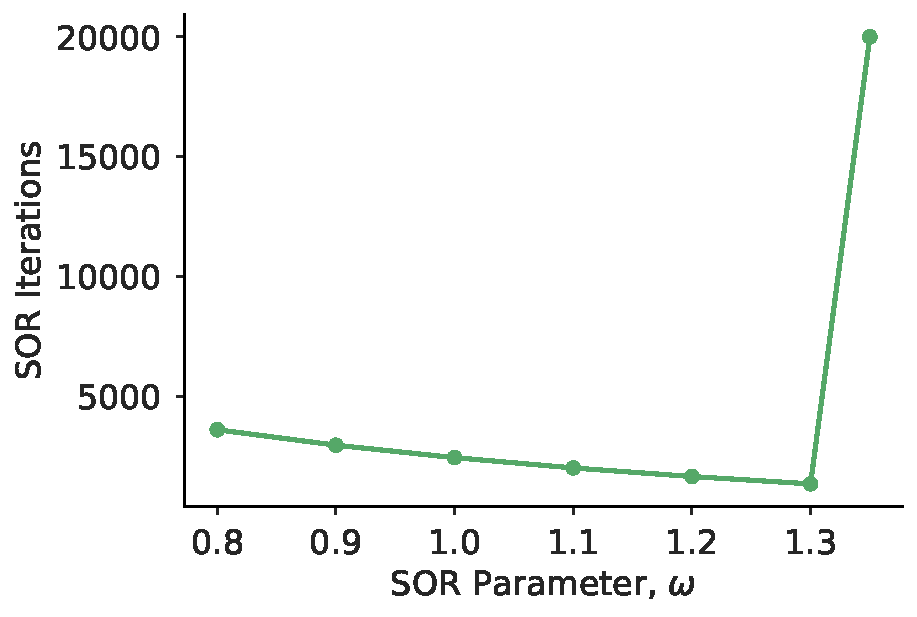
\includegraphics[width=.5\textwidth]{smith_fig8.pdf}
    \caption{Performance of the SOR algorithm for various settings of $\omega$
        using 10 samples, $\rangeh=10$, tolerance of $10^{-15}$, and $M=1$.
    }
    \label{fig:sor}
\end{figure}

We find this simple implementation to be an effective method for solving the
linear system.
\cref{fig:sor} shows the number of iterations required for
convergence as a function of the parameter $\omega$, with an optimal value of
approximately $\omega^*=1.3$.
We note that the number of iterations required to converge at this optimal value
is about half that of $\omega=1$, which coincides with a (block) Gauss-Seidel algorithm
(again differing from it's true form due to the halo updates).
Of course, \cref{fig:sor} shows the major drawback of the SOR algorithm: near
the ``optimal'' value for the SOR parameter, efficiency is highly sensitive.
For our implementation, at $\omega=1.35$, we see that the algorithm does not
fully converge and runs until set limit of 20,000 iterations.

\section*{Acknowledgements}

I am grateful to Vikram Garg early discussions on the
work by \citet{RSSB:RSSB777}, and to Jemima Tabeart for introducing me to the
implicit diffusion operator developments by \citet{mirouze_representation_2010}.
I thank Patrick Heimbach, Michael Diamond, Michael MacFerrin, and Fangfang Yao
for comments which improved the manuscript.

\bibliography{references}
\end{document}
